\chapter{Implementing a Parser for \Beluga}

This chapter presents an overview of parsing and explains the motivation behind the contributions made to \Beluga's and \Harpoon's parsing algorithms.
Some aspects of context-sensitive disambiguation of \acp{AST} are showcased, including grammars for parsing user-defined prefix, infix and postfix operators.

\section{Introduction}

This section provides a conceptual introduction to parsing, a discussion on the concept of ambiguity in parsing, and finally an overview of concepts and features of parsers for programming languages in proof assistants.
Notably, we motivate the introduction of semantic analysis as part of syntactic analysis when it comes to resolving ambiguities in a language such as \Beluga.

% What is parsing?

In compiler design, parsing is the process of converting the textual representation of a program into a hierarchical data structure~\cite{aho2007compilers, afroozeh2019practical}, which is typically called a parse tree.
When a parse tree captures all the data about the text being processed, including comments and parentheses, then it is referred to as a concrete syntax tree.
Otherwise, when parts of the data have been abstracted away, it is instead called an \ac{AST}.

% What is ambiguity in parsing?

A program's textual representation is ambiguous with respect to a predefined set of parse rules if the program can be parsed into multiple parse trees~\cite{aho2007compilers} (also called a parse forest).
By way of analogy, a sentence in a natural language is ambiguous if it can be interpreted in multiple valid ways with respect to its syntactic and grammatical rules.
Since programming languages are tools for describing computerized systems, it is necessary that each valid written program has exactly one interpretation~\cite{aho2007compilers}.
In the strictest of cases, this unicity of interpretation may be enforced at the level of the parser, such that all valid programs have exactly one inferable interpretation.
This is typically achieved using rules and syntactic conventions that prevent ambiguous programs from being ever written in the first place.

Certain kinds of syntactic ambiguities are unavoidable in programming languages, and are frequently useful to the end user.
Indeed, programming languages often reuse or overload syntactic constructs to reduce both the number and the complexity of rules that users have to learn in order to read and write programs.
Ambiguous syntax can also make programs more terse, which may improve some workflows.
Additional mechanisms need to be put in place as part of the compiler's implementation to detect syntactic ambiguities, and either signal them as errors, or resolve them using additional interpretation rules.

% What is disambiguation in parsing?

Disambiguation is the process by which a parse forest is filtered down to a single parse tree.
It refers to the procedures used to resolve ambiguities in the result of parsing.
In parsing systems that do not output parse forests, disambiguation typically involves manipulating the \ac{AST} representation of a single parse tree that captures ambiguities, meaning that some of its nodes represent the overlapping of syntactic constructs.
Functionally, these nodes suspend parsing until more information is available to disambiguate them to the correct node variant.

% What is the impact of disambiguation on program readability?

Increasing the amount of computation required to disambiguate the textual representation of a program negatively impacts the maintainability and readability of that program for the end user.
Indeed, some forms of ambiguity in the syntax of a program may prevent the end user from fully understanding it in isolation from the rest of the compilation units.
As such, one can argue that the programmatic strategies for disambiguating the syntax of a programming language should be intuitive.
For instance, name resolution is sufficiently intuitive for an end user to perform as they read the program, whereas searching in a parse forest for a parse tree that type-checks is not intuitive.

Different kinds of concrete syntax ambiguities may arise during parsing of a programming language.
We distinguish three kinds of syntactic ambiguities that come into play in the implementation of \Beluga, listed below in increasing level of computational complexity required to solve them:
\begin{enumerate}
\item
Static operator ambiguities: operators and their operands may be interpreted in different orders depending on where they appear in a whitespace-delimited list of terms.
%For instance, the expression $a + b * c$ is ambiguous with respect to the production rules $e\coloneqq e+e\mid e*e$.
These ambiguities are typically resolved by assigning a precedence level, a fixity and an associativity to each operator in the language, and parsing them as keywords.
\item
Name-based ambiguities: overloaded identifiers may be resolved to different binding sites depending on where they appear in an expression.
Semantic analysis of the \ac{AST} with respect to a symbol table is usually sufficient in those cases.
However overloading of identifiers in mixfix operators pose additional challenge since identifiers may not be considered in isolation.
\item
Type-based ambiguities: the correct interpretation of an expression may only be determined once a type has been inferred for it.
This does not refer to method overloading in object-oriented programming languages since the syntax for calling a method is not ambiguous.
Rather, if the expression being parsed is an identifier, then a type-based ambiguity may be that that expression or a surrounding one falls into a different syntactic category based on the identifier's type or kind.
In those cases, some type information may be provided by a symbol table if the type ascribed to an identifier is known at the declaration site.
In general it is impossible to disambiguate expressions having type-based ambiguities before type-checking, especially when more intricate type inference algorithms need to be applied to determine the type of an identifier.
\end{enumerate}

% TODO: Figure showcasing typical ambiguities

% What is the typical workflow for designing syntaxes and implementing parsers? What are parser generators? What are their limitations?

Typically, language designers specify the concrete syntax of their language using a \ac{CFG}, which they denote in \ac{EBNF}.
If a language can be specified by a \ac{CFG}, then we say that it is a \ac{CFL}.
\Acp{CFL} have many advantages, including the fact that there is an abundance of battle-tested parser generators for such languages.
Crucially, \acp{CFL} are easy to parse, both by the parsing algorithm and by the end user.
As the name suggests, a \ac{CFL} does not require, during parsing, additional data in a context specifically intended for disambiguation.
This ensures that programs can scale and be readable by the user without having to fully known the context in which the programs appear in order to disambiguate them.
That is, other compilation units in a \ac{CFL} do not affect how a given compilation unit is parsed.
Operator ambiguities as mentioned above can be resolved by rewriting the grammar while keeping it context-free.
The other two kinds of ambiguities however give rise to context-sensitive, or even strictly Turing-recognizable, languages~\cite{chomsky1956three}.
As the name suggests, context-sensitive languages necessitate additional data about the context in which parts of the program appears in order to parse it.
This typically implies that some semantic analysis needs to be performed during parsing in order to complete the syntactic analysis.
Consequently, the concrete syntax's design for a programming language is intrinsically linked with the algorithm required to parse it.

% What are some language design considerations?

We say that a grammar is dynamic (or user-extensible, or featuring syntax extensions) if the way a program is parsed is influenced by directives in the program itself, and otherwise we say that the grammar is static.
Languages for specifying logics tend to favour user-extensible grammars over static ones.
Indeed, \Agda and \Isabelle/\HOL support mixfix operators, \Coq has notation declarations, and \Beluga, like \Twelf, has prefix, infix and postfix operators specified by pragmas.
This is justified by the need for more concise and expressive ways to convey the meaning of definitions and lemmas.
Such syntax extensions also allow users to develop mechanizations with notations that are closer to what appears on pen-and-paper proofs.
However, that design choice negatively impacts the implementation of external tools for the language.
Indeed, user-defined syntax extensions complicate the implementation of incremental parsing for efficiently parsing edits in a text editor, as well as indexing for resolving identifiers to their binding site.
%This is notably the case for tooling in \textsc{C++} because of its rich pre-processor that increases the complexity of parsing and name resolution.

Early versions of the \Beluga language were context-free and used \textsc{Camlp4}~\cite{de2003camlp4} as parser generator for implementing its parser.
\Beluga became context-sensitive when modifications were made to its syntax, specifically for contextual objects and the addition of user-defined operators as in \Twelf for \LF type-level and term-level constants.
These changes did not pose a problem with the parser's implementation per se, but it did require the introduction of a disambiguation phase, or rather the inclusion of syntactically ambiguous nodes in the signature reconstruction algorithm.
Specifically, parts of indexing and reconstruction, as illustrated in figure~\ref{figure:legacy-beluga-processing-pipeline}, and the elaboration steps in between, had to be implemented with overlapped \ac{AST} node variants.

% What are parser combinators? What are some well-known libraries for parser combinators? What are their limitations?

As the \Beluga language grew, so did the complexity of its grammar, such that the errors generated by \textsc{Camlp4} were deemed not sufficiently informative to the end-user.
Hence, \Beluga version \texttt{1.0.0} featured a new parser implemented using monadic parser combinators, which are higher-order functions for constructing top-down recursive descent parsers~\cite{Burge1975-BURRPT, hutton1996monadic, leijen2001parsec, generalparsercombs}.
They provide a more declarative way of constructing complex parsers than shift-reduce parsers.
Indeed, the combination of smaller parsers in \OCaml using operators closely resembles grammar specifications using \acp{CFG}, which allows for fast prototyping and better readability of the implementation.
The intent of re-implementing \Beluga's parser to use parser combinators was to improve error-reporting for the end user, and to improve the overall maintainability of the implementation for subsequent developers.
These objectives were largely met, and as a consequence \Harpoon was also implemented using that parsing framework.
Nonetheless, there is still room to improve in the way of user-friendly error messages to help newcomers get a better grasp of the language and its features.

% TODO: Note that the parser before Jake's had mix/unmix types.
% TODO: Read "Resolvable Ambiguity" https://arxiv.org/pdf/1911.05672.pdf

% TODO: Define notation-based ambiguities (precedence, fixity, associativity)
% TODO: Define scope-based ambiguities (identifier classes, mutual recurrences)
% TODO: Define type-based ambiguities (identifier classes, extrinsics, type reconstruction)

% TODO: Define stateless and stateful ambiguity resolutions

% TODO: Does Abella support incremental development?
% TODO: See if Agda breaks with splicing
% TODO: See if Coq has incremental development as well

% TODO: Literary review of data-dependent parsing, curtailing

\section{\Beluga Lexing, Parsing and Disambiguation Phases}

\Beluga's parser was re-implemented to handle expressions in non-normal form, to support user-defined operators at the level of computations, and to improve the implementation's maintainability.
Particularly, semantic analysis is introduced as part of a new context-sensitive disambiguation phase to the parser in order to produce a fully unambiguous \ac{AST} before signature reconstruction.
Additionally, support for incremental program development was added using architectural refactoring techniques.

The motivation for these changes to the implementation can be summarized in the following points:
\begin{enumerate}
\item
Expand the operator pragmas feature to computation-level types and expressions.
This involved the implementation of a reusable process for disambiguating function applications denoted by the juxtaposition of terms.
\item
Improve syntax error messages.
By accepting a wider range of programs during parsing, the subsequent disambiguation phase can more precisely identify the cause for syntax errors and report them with better detail.
\item
Improve the parser's maintainability.
By decoupling disambiguation from indexing, both phases now respect the single-responsibility principle, which in turn simplifies the information flow at the early stage of signature reconstruction.
\item
Provide verifiably-correct external \acp{AST} to enable debugging of signature reconstruction.
Since the disambiguated external \ac{AST} of a program fully captures the meaning of what the user wrote, then the internal \ac{AST} as illustrated in figure~\ref{figure:legacy-beluga-processing-pipeline} is no longer the only complete data representation of the program.
\end{enumerate}

The revised parsing algorithm for \Beluga signatures is split into three phases, namely: lexing, parsing and disambiguation, which are outlined in the following sections.
First, lexing is implemented just like in typical whitespace-agnostic programming languages, except for one lexer hack used to handle some overloading of a static operator.
Then, parsing produces an \ac{AST} close to the concrete syntax, and featuring ambiguous nodes that effectively postpone parsing steps that require data for the referencing environment at a given node.
Finally, disambiguation converts the parsed \ac{AST} to a revised external \ac{AST} without ambiguous nodes.

\subsection{Lexing}

Lexical analysis for \Beluga uses regular expressions to convert sequences of characters into tokens to speed up recursive descent parsing.
Sections~\ref{section:comments-lexical-convention}, \ref{section:keywords-lexical-convention} and \ref{section:lexical-convention} provide the functional requirements for this phase of the implementation.
Notably, lexing of nested delimited comments (i.e., those comments enclosed in either \verb|%{| and \verb|}%|, or \verb|%{{| and \verb|}}%|) is achieved by parameterizing with respect to the depth of the comment.
This ensures that extraneous or missing right-delimiters are detected early.

Where the lexing phase diverges from conventional implementations is with regards to the dot operator.
Indeed, usual lexical conventions dictate that whitespace may precede or follow a dot without affecting a program's semantics.
This cannot apply in \Beluga programs, where a dot denotes one the following:
\begin{enumerate}
\item
The end of an \LF term-level or type-level constant declaration, like in \Twelf.
\item
The beginning of a computation-level observation application for coinductive objects.
\item
The delimiter between the parameter name and the body of an \LF $\lambda$-abstraction.
\item
The projection out of a contextual \LF block term.
\item
The projection out of a computation-level tuple expression.
\item
The projection out of a module acting as a namespace.
\end{enumerate}

% TODO: Describe the lexer hack for the dot operator
% TODO: Read "Rating Disambiguation Errors"

\subsection{Parsing}

Parsing of \Beluga signatures is achieved using $ \mathsf{LALR(\infty)} $ parsing in pathological cases and $ \mathsf{LALR(1)} $ parsing in the most frequent cases.
This is implemented using the monadic parser combinator library introduced in \Beluga version \texttt{1.0.0}.
Unlimited backtracking of the parser state is enabled only in select cases, or if no input token has been consumed, which provides sufficient performance for parsing large \Beluga files.

The main contribution made to the context-free parsing phase of \Beluga is the simplification of its grammar.
Indeed, the legacy parser was designed following the grammars developed along signature reconstruction and type-checking algorithms, which introduced syntactic classes that ensure some properties always hold.
Specifically, the index level \LF of \Beluga is strongly-normalizing, and since reconstruction for \LF terms and types operates best with objects in canonical form, then it was decided that the user should only be able to write \LF terms and types in canonical form.
This required that parser productions be introduced for normal and neutral terms separately.
Additionally, since \Beluga's type-checking algorithm is bidirectional, computation-level expressions were split into two syntactic classes, namely type-synthesizing expressions and type-checkable expressions, and this change was also reflected in the parser.
Implementation efforts revealed however that these syntactic constraints are too stringent to be imposed during parsing.
Indeed, they increased the complexity of the parser, made operator precedence rules opaque, and yielded poor syntax error messages to the user.
The pre-terms of \Beluga cannot be elegantly partitioned all at once by order of precedence, by whether they are neutral or normal, and whether they synthesize a type or check against one.
Those rules for parsing are too complex to be explained to newcomers to the language, and are also error-prone for developers.
The additional constraints further restrict the language recognized by the parser, which in turn prevents some syntactically invalid programs from being reported beyond identifying unexpected tokens.
This is in part evidenced by the grammar in figure~\ref{figure:legacy-clf-parsing} and the example syntax error message in figure~\ref{figure:improved-syntax-error-message}.

\begin{figure}[H]
\begin{grammar}
<clf-normal> ::=
     `\\' <identifier> `.' <clf-term-application>
\alt `(' <clf-term-application> [`:' <clf-type>] `)'
\alt <hash-identifier> [<clf-projection>] [ `[' <clf-substitution> `]' ]
\alt <qualified-identifier> [<clf-projection>] [ `[' <clf-substitution> `]' ]
\alt `_'
\alt `?'<identifier>
\alt `<' <clf-term-application> (`;' <clf-term-application>)+ `>'

<clf-projection> ::=
     `.' <integer>
\alt `.' <identifier>

<clf-term-application> ::=
     <clf-normal>+
\alt <clf-type>

<clf-type> ::=
     `{' <identifier> `:' <clf-type> `}' [`->'] <clf-type>
\alt <clf-type-atomic> [`->' <clf-type>]

<clf-type-atomic> ::=
     <clf-normal>+
\alt <identifier> <clf-normal>*
\alt `(' <clf-type> `)'
\alt `block' `(' <identifier> `:' <clf-type> (`,' <identifier> `:' <clf-type>)+ `)'
\end{grammar}
\caption[The grammar for parsing contextual \acs{LF} terms in normal form in the legacy parser.]{%
The grammar for parsing contextual \LF terms in normal form in the legacy parser, denoted using the lexical conventions of section~\ref{section:lexical-convention}.
The production \synt{clf-substitution} is omitted for brevity.
The productions \synt{clf-term-application} and \synt{clf-type-atomic} showcase a dramatic increase in complexity for parsing contextual \LF terms and types.
This presentation also does not effectively demonstrate that left recursions never occur, and what precedence each operator has.
}
\label{figure:legacy-clf-parsing}
\end{figure}

\begin{figure}[H]
\begin{subfigure}{\linewidth}
\begin{Verbatim}[commandchars=\\\{\}, baselinestretch=1]
exp : \verbbf{type}.
eq : exp -> exp -> \verbbf{type}.
\verbbf{schema} ctx = \verbbf{block} (x : exp, t : eq x x);
\verbbf{rec} reflexivity : \{g : ctx\} \{M : [g |- exp]\} [g |- (eq M M)[..]] = ?;
\end{Verbatim}
\caption{%
Example \Beluga theorem statement with a syntactically invalid substitution.
The identity substitution \texttt{[..]} on the application of an \LF type constant in \texttt{(eq M M)[..]} is invalid because only canonical forms of \LF objects are recognized for signature reconstruction.
}
\end{subfigure}
\par\bigskip
\begin{subfigure}{\linewidth}
\begin{Verbatim}[baselinestretch=1]
example.bel, line 5, column 59:
Parse error.
Unexpected token in stream
  Expected token `]'
  Got token `['
\end{Verbatim}
\caption{%
Syntax error raised during context-free parsing in the previous parser implementation.
Given the stricter grammar of \synt{clf-type} in figure~\ref{figure:legacy-clf-parsing}, it is true that the token \texttt{[} introducing the identity substitution is unexpected.
However, the reason for this syntax error is not obvious, in part because the user unambiguously wrote a substitution.
}
\end{subfigure}
\par\bigskip
\begin{subfigure}{\linewidth}
\begin{Verbatim}[commandchars=\\\{\}, baselinestretch=1]
\verbpbf{File "example.bel", line 5, column 52:}
5 |rec reflexivity : \{g : ctx\} \{M : [g |- exp]\} [g |- (eq M M)[..]] = ?;
                                                      \verbrbf{^^^^^^^^^^^^}      
\verbrbf{Error:} Substitution terms may not appear as contextual LF types.
\end{Verbatim}
\caption{%
Improved syntax error message produced during the disambiguation phase instead of during context-free parsing.
Since the grammar for \LF objects was relaxed to support non-canonical forms, the parser accepts the invalid substitution, and then disambiguation identifies that it should be rejected.
}
\end{subfigure}
\caption[Example of improved syntax error reporting]{%
Example of improved syntax error reporting using less stringent syntactic rules at the level of the parser.
}
\label{figure:improved-syntax-error-message}
\end{figure}

Besides the aforementioned simplifications to the grammar, the revised parser still had to support the syntax of \LF kinds, types and terms, which overloads operators.
In fact, an \LF kind is syntactically indistinguishable from an \LF type in \Beluga until the very last operand to the arrow operator.
Unrestricted backtracking and infinite lookaheads are not suitable solutions to this disambiguation issue given that those expressions are the most frequent ones in \Beluga signatures.
The solution we employ to resolve this issue of complexity during context-free parsing is somewhat counter-intuitive.
We merge syntactic categories having common syntaxes that appear in ambiguous positions into a single production.
We call this blurring the grammar since we effectively lose the distinction between syntactic categories during context-free parsing.
Section~\ref{section:blurred-lf-syntax} provides an example of one such blurred grammar, obtained by merging the productions \synt{lf-kind}, \synt{lf-type} and \synt{lf-term} of section~\ref{section:syntax-lf} into one syntactic category, with corresponding production \synt{lf-object}.
The context-sensitive disambiguation phase outlined in the next section is then tasked with recovering the original \LF kind, type or term corresponding to a parsed \LF object.
We note that a similar technique was used in \Twelf since its shift-reduce parser could not perform disambiguation during parsing.

\subsection{Disambiguation}

The disambiguation phase of parsing statefully keeps track of the identifiers in scope at any given point during a traversal of the parser \ac{AST}.
This is implemented using a mutable state with auxiliary data structures to deal with patterns, modules and pragmas.
Specifically, bindings during this phase are modelled using a stack of scopes, each of which contains a tree mapping fully qualified identifiers to minimal descriptions of bound variables and constants.

We postpone the discussion on how the referencing environment is constructed and updated during the \ac{AST} traversal to section~\ref{section:indexing} because it closely follows the procedure used to compute de Bruijn indices during the indexing phase.

% TODO: Figure illustrating the semantic analysis of names during disambiguation

% TODO: Prove the unicity of disambiguation for the pure LF level, using a stepping relation indexed by the precedence level for applications

\section{Parsing User-Defined Operators}

In \Beluga, users may specify that identifiers should be used as operators in expression applications, as shown in figure~\ref{figure:operator-pragmas}, using \verb|--prefix|, \verb|--infix| or \verb|--postfix| pragmas.
Prefix operators are right-associative, postfix operators are left-associative, and infix operators may be either left-associative, right-associative or non-associative.
The priority of operations can be specified using integer precedence values.
This feature was ported over from \Twelf, and using the new parsing architecture, it was subsequently improved to support shadowing of operators by bound variables.
As outlined below, the notation pragmas for user-defined operators in \Beluga are more restrictive than that of \Agda because \Beluga does not support mixfix operators~\cite{danielsson2008parsing}.

\begin{figure}[H]
\begin{Verbatim}[commandchars=\\\{\}, baselinestretch=1]
\verbbf{LF} p : \verbbf{type} =
| \makebox[1em]{⊃} : p \makebox[1em]{→} p \makebox[1em]{→} p                  \verbcomment{% Logical implication}
| \makebox[1em]{⊂} : p \makebox[1em]{→} p \makebox[1em]{→} p                  \verbcomment{% Converse implication}
| \makebox[1em]{∧} : p \makebox[1em]{→} p \makebox[1em]{→} p                  \verbcomment{% Logical conjunction}
| \makebox[1em]{∨} : p \makebox[1em]{→} p \makebox[1em]{→} p                  \verbcomment{% Logical disjunction}
| \makebox[1em]{¬} : p \makebox[1em]{→} p                       \verbcomment{% Logical negation}
| \makebox[1em]{⊤} : p                            \verbcomment{% Tautology}
| \makebox[1em]{⊥} : p                            \verbcomment{% Contradiction}
;
\verbprag{--infix \makebox[1em]{⊃} 3 right.}    \verbcomment{% Subsequently treat ⊃ as a right-associative}
\verbprag{--infix \makebox[1em]{⊂} 3 left.}     \verbcomment{% infix operator with precedence value 3}
\verbprag{--infix \makebox[1em]{∧} 5 right.}
\verbprag{--infix \makebox[1em]{∨} 4 right.}
\verbprag{--prefix \makebox[1em]{¬} 10.}

\verbbf{let} a = [x : p ⊢ ¬ ¬ ¬ x]
\verbbf{let} b = [x : p, y : p ⊢ ¬ x ⊂ y ⊂ ⊥]
\verbbf{let} c = [x : p, y : p, z : p ⊢ ⊤ ∨ x ∧ ¬ y ⊃ ¬ z]
\verbbf{let} d = [f : p \makebox[1em]{→} p, x : p ⊢ ¬ f x ∨ f ⊥]
\end{Verbatim}
\caption[Example of user-defined operator definitions in \Beluga using pragmas.]{%
Example of user-defined operator definitions in \Beluga using pragmas.
The subsequent meta-objects \texttt{a}, \texttt{b}, \texttt{c} and \texttt{d} use those notations to construct formulas just like in proofs on paper.
}
\label{figure:operator-pragmas}
\end{figure}

\begin{figure}
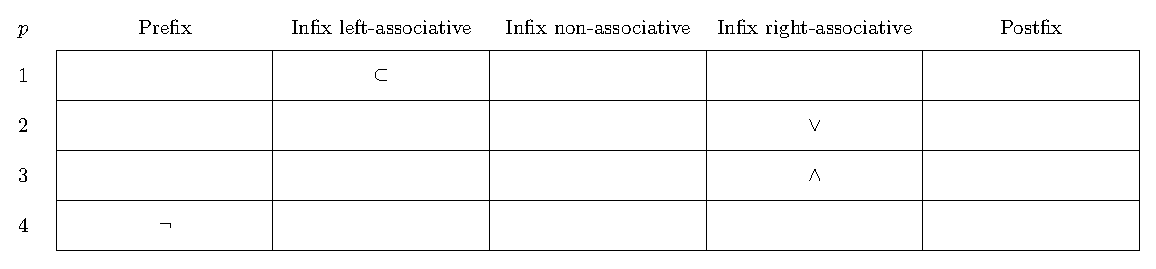
\includegraphics[width=\textwidth]{figures/operator-table.eps}
\caption[Example operator table for parsing user-defined operators.]{%
Example operator table for parsing user-defined operators for applications containing the operators $\lnot$, $\land$, $\lor$ and $\subset$ from figure~\ref{figure:operator-pragmas}.
For instance, this table would be used to parse $x \subset x \lor y \lor \lnot z \land w$ as $x \subset (x \lor (y \lor ((\lnot z) \land w)))$.
}
\label{figure:operator-table}
\end{figure}

The legacy \Beluga system only supported user-defined operators for \LF type-level and term-level applications.
As such, only constants in \LF could be defined as operators.
The proposed revisions allow for user-defined operators to be used in all applications, meaning that computation-level types and expressions may also benefit from prefix, infix and postfix notations.
Specifically, all typed constants can now be annotated with a notation pragma.

The new implementation for parsing user-defined operators relies on the disambiguation phase for resolving identifiers to constants and their notations.
As such, the initial parser suspends parsing of applications, meaning that it represents the juxtaposition of parsemes as lists.
Disambiguation then resumes parsing with a recursive descent parser instantiated specifically for the constants that appear in the list of parsemes.
That is, when disambiguating an application node, not all constant declarations in scope at that point in the \Beluga signature need to be taken into account.
We only need to build an operator table as in figure~\ref{figure:operator-table} for the operators appearing in the application.
This ensures that the complexity of this second phase of parsing for applications scales only with the number of parsemes in the list, and not with the size of the signature.
However, this design requires that operators cannot be overloaded, otherwise disambiguation of applications could only be realized when type information is available, which happens much later in signature reconstruction for \Beluga.

In \Beluga, at the precedence level of expression applications, there are four scenarios to disambiguate:
\begin{enumerate}
\item Prefix operators followed by their operand,
\item Left-associative, right-associative or non-associative infix operators preceded and followed by their operands,
\item Postfix operators preceded by their operand, and
\item Juxtaposed expressions having no operator.
\end{enumerate}

During the disambiguation phase of parsing, we only need to determine the syntactic structure of applicands and arguments for parsemes in lists.
The implementation of this parsing algorithm is inspired by the general purpose expression parser from the \texttt{Parsec} library~\cite{leijen2001parsec}, as well as the parser scheme in figure~\ref{figure:user-defined-operators-grammar}, which is inspired by the one found in~\cite{danielsson2008parsing}.
This parsing algorithm proceeds in the following steps:
\begin{enumerate}
\item Identify the constants with user-defined operator notations in the list of parsemes.
\item Group those identifiers by precedence, then by fixity and associativity, like in the table in figure~\ref{figure:operator-table}.
\item Construct a parselet for each precedence level in the operator table, such that the precedence climb delegates parsing to the parselet for the next precedence level, in increasing order.
\item Run the parselet handling the least precedence level on the list of parsemes.
\end{enumerate}
This is effectively the same principle as recursive descent parsing for a set of operators statically defined by the language's grammar, but instead implemented over a dynamic set of operators.
This set is constructed using only those constants found in the \ac{AST} node for application.
As such, this parsing algorithm for user-defined operators has $ O(n^3) $ runtime complexity, where $ n $ is the length of the list of parsemes.
Figures~\ref{figure:user-defined-operators-initial-grammar}, \ref{figure:user-defined-operators-initial-grammar-scheme} and \ref{figure:user-defined-operators-final-grammar-scheme} progressively show how to obtain a grammar scheme for implementing parsing of user-defined operators.
This parser is implemented following the last grammar scheme, and using monadic parser combinators just like in the context-free parsing phase.

Coincidentally, the grammar scheme of figure~\ref{figure:user-defined-operators-initial-grammar-scheme} was used to reintroduce support for infix left and right arrow operators $\rightarrow$ and $\leftarrow$ in \LF types.
% TODO: Talk about restrictions on what operators can appear at the same precedence level
% TODO: Recap table for supported operators


{\newcommand{\prefix}{\mathsf{op}_{\text{prefix}}}
\newcommand{\infix}{\mathsf{op}_{\text{infix}}}
\newcommand{\infixl}{\mathsf{op}_{\text{infix}}^L}
\newcommand{\infixr}{\mathsf{op}_{\text{infix}}^R}
\newcommand{\infixn}{\mathsf{op}_{\text{infix}}^N}
\newcommand{\postfix}{\mathsf{op}_{\text{postfix}}}
\begin{figure}[H]
\begin{subfigure}{\linewidth}
\centering
\begin{tabular}{rrl}
$ \angled{e} $ & $ \Coloneqq $ & $ \angled{\prefix} \; \angled{e} $\\
& $ \mid $ & $ \angled{e} \; \angled{\infix} \; \angled{e} $\\
& $ \mid $ & $ \angled{e} \; \angled{\postfix} $\\
& $ \mid $ & $ \mathbf{a}+ $
\end{tabular}
\caption{Ambiguous grammar for parsing user-defined operators. The terminal $ \mathbf{a} $ stands for expressions that were already parsed at a higher precedence level than any user-defined operator during the context-free parsing phase.
For instance, $ \mathbf{a} $ can stand for variables and projections.}
\label{figure:user-defined-operators-initial-grammar}
\end{subfigure}
\par\bigskip
\begin{subfigure}{\linewidth}
\centering
\begin{tabular}{rrl}
$ \angled{e} $ & $ \Coloneqq $ & $ \angled{e}_1 $\\
$ \angled{e}_p $ & $ \Coloneqq $ & $ \angled{e}_{p + 1} \; \angled{\infixn}_p \; \angled{e}_{p + 1} $\\
& $ \mid $ & $ \left(\angled{\prefix}_p \mid \angled{e}_{p + 1} \; \angled{\infixr}_p\right)\hspace{-0.3em}{+} \; \angled{e}_{p + 1} $\\
& $ \mid $ & $ \angled{e}_{p + 1} \; \left(\angled{\postfix}_p \mid \angled{\infixl}_p \; \angled{e}_{p + 1}\right)\hspace{-0.3em}{+} $\\
& $ \mid $ & $ \angled{e}_{p + 1} $\\
$ \angled{e}_{P + 1} $ & $ \Coloneqq $ & $ \mathbf{a}+ $
\end{tabular}
\caption{%
Initial grammar scheme for parsing user-defined operators.
$ P $ is the number of distinct precedence levels induced by the user-defined operators appearing in the application, and $ \angled{e}_p $ is the production for an expression at precedence level $ p $.
Similarly, $ \angled{\infixn}_p $, $ \angled{\infixr}_p $ and $ \angled{\infixl}_p $ stand for infix non-associative, right-associative, and left-associative operators respectively, all at precedence level $ p $.
}
\label{figure:user-defined-operators-initial-grammar-scheme}
\end{subfigure}
\caption[Grammars for parsing user-defined operators in \Beluga.]{Grammars for parsing user-defined operators in \Beluga.}
\label{figure:user-defined-operators-grammar}
\end{figure}%
\begin{figure}\ContinuedFloat
\begin{subfigure}{\linewidth}
\centering
\begin{tabular}{rrl}
$ \angled{e} $ & $ \Coloneqq $ & $ \angled{e}_1 $\\
$ \angled{e}_p $ & $ \Coloneqq $ & $ \angled{\prefix}_p \; \angled{e_r}_p $\\
& $ \mid $ & $ \angled{e}_{p + 1} \; \angled{e_t}_p $\\
$ \angled{e_t}_p $ & $ \Coloneqq $ & $ \angled{\infixn}_p \; \angled{e}_{p + 1} $\\
& $ \mid $ & $ \angled{\infixr}_p \; \angled{e_r}_p $\\
& $ \mid $ & $ \angled{\infixl}_p \; \angled{e}_{p + 1} \; \angled{e_l}_p $\\
& $ \mid $ & $ \angled{\postfix}_p \; \angled{e_l}_p $\\
& $ \mid $ & $ \varepsilon $\\
$ \angled{e_l}_p $ & $ \Coloneqq $ & $ \angled{\postfix}_p \angled{e_l}_p $\\
& $ \mid $ & $ \angled{\infixl}_p \angled{e}_{p + 1} \angled{e_l}_p $\\
& $ \mid $ & $ \varepsilon $\\
$ \angled{e_r}_p $ & $ \Coloneqq $ & $ \angled{\prefix}_p \angled{e_r}_p $\\
& $ \mid $ & $ \angled{e}_{p + 1} \angled{e_r'}_p $\\
$ \angled{e_r'}_p $ & $ \Coloneqq $ & $ \angled{\infixr}_p \angled{e_r}_p $\\
& $ \mid $ & $ \varepsilon $\\
$ \angled{e}_{P + 1} $ & $ \Coloneqq $ & $ \mathbf{a}+ $
\end{tabular}
\caption{Factored grammar scheme derived from figure~\ref{figure:user-defined-operators-initial-grammar-scheme} for parsing user-defined operators. The parser implementation using that grammar may additionally intersperse failure productions to peek at the next token in the input stream and raise an exception if that token is an operator in an ambiguous position.}
\label{figure:user-defined-operators-final-grammar-scheme}
\end{subfigure}
\caption[]{Grammars for parsing user-defined operators in \Beluga (cont.).}
\end{figure}}

\section{Discussion}

Despite the bugfixes and new features, the revised parser architecture is not without its flaws.
The additional requirement that parsing must produce an unambiguous \ac{AST} prevents the overloading of some syntax.
In particular, meta-objects and meta-types for substitutions had to be prefixed by \texttt{\$} to distinguish them from plain meta-objects and meta-types respectively.
For the same reason, parameter meta-types had to be prefixed by \texttt{\#}.
Those breaking changes to the syntax could have been avoided had further semantic analysis been introduced during the disambiguation phase, namely to perform type-driven disambiguation.
Should \Beluga be extended to support multiple context variables in contexts, then this may be required.

% TODO: Agda embraces ambiguity, and spreads ambiguities across more syntaxes https://agda.readthedocs.io/en/v2.6.2.2/language/core-language.html#:~:text=The%20syntax%20of%20an%20Agda,Pragmas%20define%20program%20options.
